%%--------------------------------------
%% DEFINITIONS
%%--------------------------------------

\nonstopmode

%% Font 12pt
%% Paper A4
%% Language englanti
%% Left-justify equation numbering
\documentclass[12pt,a4paper,english,leqno]{article}

\usepackage{natbib}
\bibpunct{(}{)}{;}{a}{,}{,}

\usepackage[T1]{fontenc}
\usepackage[utf8]{inputenc}
\usepackage[english]{babel}
\usepackage{graphicx}
\usepackage{xcolor}
\usepackage{url}


%% Use palantino as font
\usepackage[osf,sc]{mathpazo} 

%% Marginals
\usepackage[a4paper,right=3cm,left=4cm,vmargin=3cm]{geometry}

%% Linespacing
\linespread{1.6}

%% Remove widow and orphan lines
\clubpenalty=10000
\widowpenalty=10000

%% Remove hyphenation
\tolerance=1
\emergencystretch=\maxdimen
\hyphenpenalty=100
\hbadness=100

\begin{document}

\parskip 2mm
\parindent 0mm

%%--------------------------------------
%% FRONTPAGE
%%--------------------------------------

\begin{titlepage}
  \setlength{\parindent}{0mm}
  \sloppy
  \large \textsc{University of Helsinki \\
  				 Faculty of Science\\
                 Department of Computer Science}
  \vspace{5mm}

  \hrule height3pt
  \vspace{20mm}

  \begin{center}
	\vfill  
  
    \begin{Huge} 
    \textbf{TestMyCode Eclipse}\\
    \end{Huge}
    \begin{LARGE}
    Project Architecture
    \end{LARGE}
    \vspace{20mm}

    \vfill

  \end{center}
  \hrule height2pt
  \vspace{5mm}

  \begin{small}
  Juhani Heliö\\
  Ville-Pekka Hämäläinen\\
  Nikke Kostiainen\\
  Erkka Kääriä\\
  Leo Leppänen\\
  Joel Nummelin\end{small} \hfill \today
  
\end{titlepage}

\tableofcontents

\pagebreak

%%--------------------------------------
%% BODY
%%--------------------------------------

\section{Overview}

The TestMyCode Eclipse plugin consists of two discrete main components: An IDE independent TestMyCode Core and an Eclipse plugin that wraps the Core component and implements necessary IDE specific features.

\section{TestMyCode Core}

\begin{figure}[ht!]
\centering
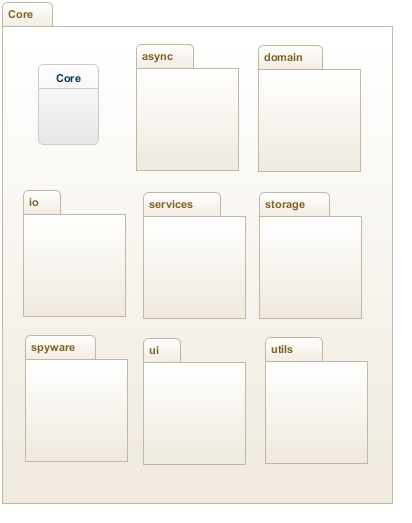
\includegraphics[scale=1]{img/core.jpg}
\end{figure}

TestMyCode Core is the IDE independent component of the project. It consists of IDE independent code that contains most of the projects logic. The Core also interfaces with other TestMyCode components such as the TestMyCode Server\footnote{https://github.com/testmycode/tmc-server} and the TestMyCode JUnit Runner\footnote{https://github.com/testmycode/tmc-junit-runner}.

\subsection{Core}

The main class of TestMyCode Core is the aptly named \textit{Core}. This class provides the actual plugin access to many other features of the core such as the user's settings, the server interface, data access objects and other core components.

\subsection{Background tasks}

\begin{figure}[ht!]
\centering
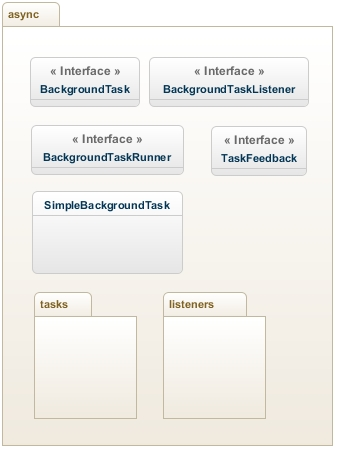
\includegraphics[scale=1]{img/async.jpg}
\end{figure}

Any actual processing the plugin needs is done asynchronously with implementations of the interface \textit{async.BackgroundTask}. Some of these tasks are associated with implementations of \textit{async.BackgroundTaskListener} that describe reactions to different states of the task.

The actual tasks are ran by an implementation of the \textit{async.BackgroundTaskRunner} that the IDE dependent plugin component needs to provide. These tasks can also invoke the IDE user interface via a IDE dependent implementation of the \textit{ui.IdeUIInvoker}.

\subsection{Input-Output}

\begin{figure}[ht!]
\centering
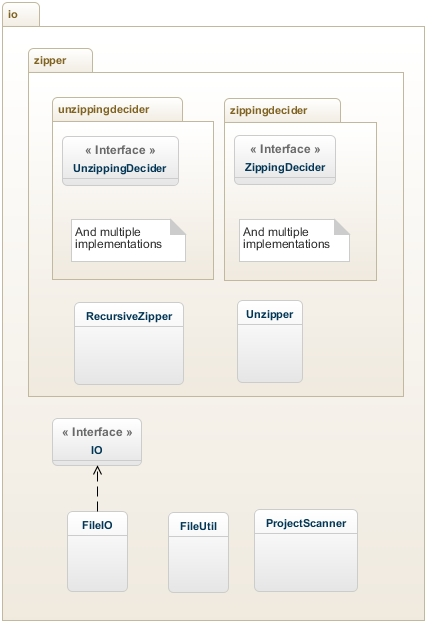
\includegraphics[scale=1]{img/io.jpg}
\end{figure}

The project needs to interface with the file system in multiple ways. We need to zip and unzip projects and save details of the exercises and projects the user has downloaded.

The package \textit{io} contains a \textit{io.FileIO} class that contains the actual logic used to interface with the file system.

For zipping and unzipping, \textit{io.zipper.RecursiveZipper} and \textit{io.zipper.Unzipper} are used. These classes utilize different implementations of \textit{io.zipper.unzippingdecider.UnzippingDecider} and \textit{ZippingDecider} that tell the zippers what files to (un)zip and what to leave untouched. This allows us to for example download full projects when updating an exercise without overwriting the student's progress.

\subsection{Services}

\begin{figure}[ht!]
\centering
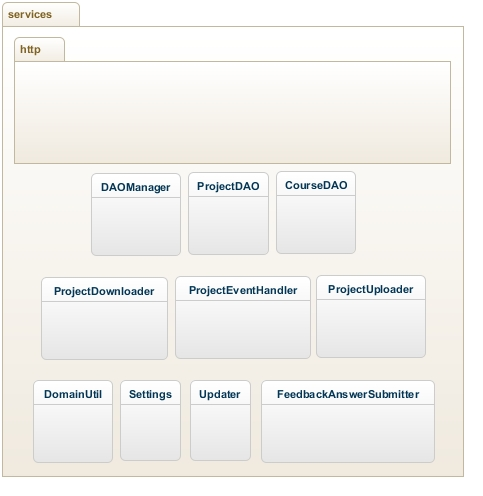
\includegraphics[scale=1]{img/services.jpg}
\end{figure}

The \textit{services} package contains our data access objects and other miscellaneous classes that other services and the plugin can utilize to accomplish different tasks.

This package also contains the subpackage \textit{services.http} that contains the code required to interface with the TestMyCode server. The main interface between this HTTP stack and other components is the \textit{services.http.ServerManager} class that provides simple methods for actions that require sending or receiving data from the TestMyCode server.

\subsection{Spyware}

The `spyware' component that resides in the \textit{spyware} package contains the logic for logging the student's actions for analysis of the student's progress and process of learning. Provided that the user has consented to sending snapshots of his study, the component sends the snapshots to TestMyCode Spyware Server\footnote{https://github.com/testmycode/tmc-spyware-server} for further analysis of the whole class' progress as a population.

This component is rather highly decoupled from the rest of the plugin and is quite self-contained. Due to being dependent of - for example - the HTTP stack, it is an integrated component of the Core instead of being a discrete project. 

The spyware component also has a `hidden' dependency to the Google diff match patch component\footnote{https://code.google.com/p/google-diff-match-patch/}. This library is provided as \textit{spyware.utility.diff\_match\_patch}. While a third party Maven implementation of the library exists, it was decided against using it until the other spyware tools are updated to utilize that as well.

\subsection{Storage}

\begin{figure}[ht!]
\centering
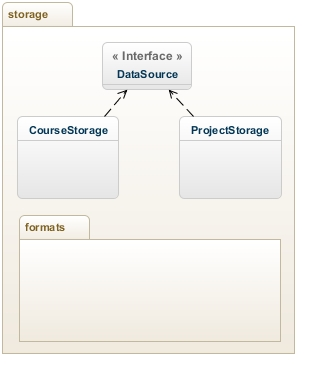
\includegraphics[scale=1]{img/storage.jpg}
\end{figure}

The \textit{storage} package contains classes that utilize the \textit{io.FileIO} to write information about the user's courses and exercises to the disk so that this information can be accessed over multiple sessions.

\subsection{User interface}

\begin{figure}[ht!]
\centering
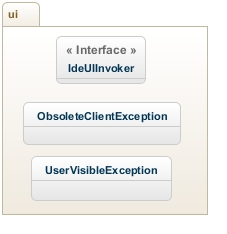
\includegraphics[scale=1]{img/ui.jpg}
\end{figure}

The \textit{ui} package mainly consists of the \textit{ui.IdeUIInvoker} interface, that the IDE specific plugin must implement. This interface defines the methods of UI-interaction that the core requires. This allows us to invoke dialogs and other UI elements from the background tasks and their listeners, allowing higher decoupling between the Core and the plugin.

\pagebreak
\section{Eclipse plugin}

\begin{figure}[ht!]
\centering
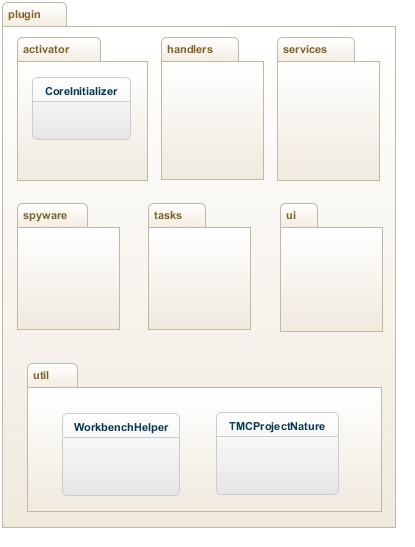
\includegraphics[scale=1]{img/plugin.jpg}
\end{figure}

The Eclipse plugin is basically an Eclipse dependent wrapper over the actual TestMyCode Core. It provides the required IDE specific implementations that are needed for the add-on to really work. The core is provided to the plugin as a shaded .jar -file, that is located in the \textit{lib/} folder.

\subsection{Activator}

The \textit{activator.CoreInitializer} defines the start-up behavior of the plugin, initializes the Core and schedules the always present background tasks such as scheduled checks for new code reviews.

\subsection{Handlers}

The package \textit{handlers} contains the classes that define how the plugin reacts to different user interface events, such as clicking on menu items. The \textit{handlers.listeners} packages contains classes that react to different user interface events, such as changing the focus. For example the class \textit{handlers.listeners.SelectionListener} allows us to disable the `submit' button whenever a non-TestMyCode project is selected.

\subsection{Services}

The package \textit{services} contains classes that open different downloaded projects in the IDE with correct project natures, f.ex. as a Maven project or as an Ant project.

\subsection{Spyware}

The \textit{spyware} package handles listening to events within the IDE editors and passes them onwards to the Core for further handling and (depending on whether the user has given consent) possibly sends the snapshot data to the TestMyCode Spyware server.

\subsection{Tasks}

The \textit{tasks} package contains the IDE specific implementations of the task running related interfaces defined by the Core.

It also contains the class \textit{tasks.TaskStarter} that contains the required logic for launching new background tasks from within the plugin component.

\subsection{User interface}

The \textit{ui} package contains all the custom dialogs and windows needed by the plugin component.

\subsection{Utilities}

The class \textit{util.WorkbenchHelper} is an utility class that contains code needed in multiple places within the plugin. It allows - for example - for resolving the `active project' (a term not native to Eclipse IDE), and saving of all open files.

Also present in the \textit{util} package is the \textit {ui.TMCProjectNature} that is used to distinguish TestMyCode projects from generic projects and allows for the status indicators in the project explorer.
\end{document}